\begin{frame}{Circle construction}

 Construct a tangent to a circle of radius 4 units
from a point on the concentric circle of radius
6 units.\\
\begin{itemize}
\item\textbf{Solution} :\\
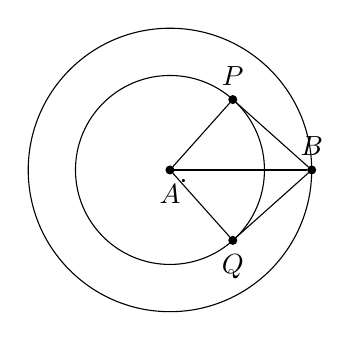
\begin{tikzpicture}
[scale =0.3,>=stealth,point/.style = {draw, circle, fill = black, inner sep = 1pt},]
\node (A) at (0,0)[point,label=below :$A$] {};
\node (P) at (2.66,2.98)[point,label=above :$P$] {};
\node (B) at (6,0)[point,label=above :$B$] {};
\node (Q) at (2.66,-2.98)[point,label=below :$Q$] {};
\draw (0,0) node [below right] {.} circle (6);
\draw (0,0) node [below right] {.} circle (4);
\draw (B)--(A);
\draw (B)--(Q);
\draw (B)--(P);
\draw (A)--(P);
\draw (A)--(Q);
\tkzMarkRightAngle[fill=white!45,size=.6,mark=](B,P,A)
\tkzMarkRightAngle[fill=white!45,size=.6,mark=](B,Q,A)
\end{tikzpicture}
\\  PB and QB are the tangents 
\end{itemize}
\seti
\end{frame}

\begin{frame}
\begin{itemize}
\item \textbf{Given} : r1=4 and r2 = 6\\
\begin{align*}
a=\sqrt{r2^2 - r1^2}\\
a=4.47\\
c=r1 and b=r2\\
p=\frac{b^2+c^2-a^2}{2b}\\
p=2.66\\
q=\sqrt{c^2 - p^2}\\
q=2.98\\
AB = r2 \\
P = (2.66,2.98)\\
Q = (2.66,-2.98)
\end{align*}
\end{itemize}

\end{frame}


\begin{frame}
\begin{figure}
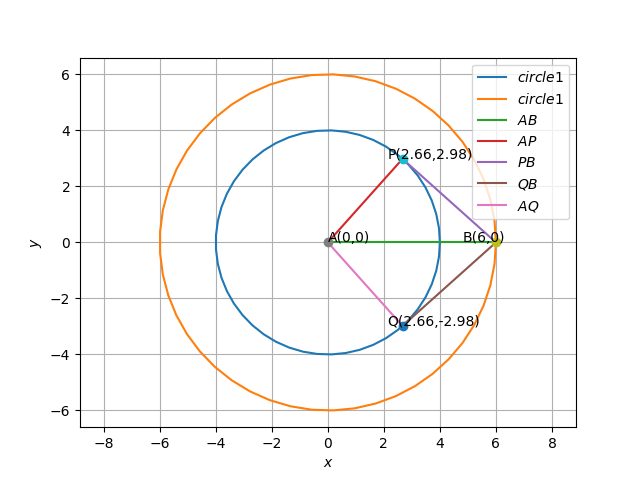
\includegraphics[scale=.4]{./CODES/circle/CIR_CON.png}
\end{figure}
\begin{itemize}
\item \url{https://github.com/pratibha444/GEOMETRY/blob/master/figs/CIRCLE_CON.tex}  \\
\item \url{https://github.com/pratibha444/GEOMETRY/blob/master/CODES/circle/circon.py}
\end{itemize}
\end{frame}